\documentclass[11pt]{article}

%----------%
% Packages %
%----------%

\usepackage{tikz}
\usepackage{fancyhdr}
\usepackage{enumitem}
\usepackage[letterpaper, margin=1in]{geometry}
\usepackage{upquote}
\usepackage[T1]{fontenc}
\usepackage{textcomp}
\usepackage{listings}
\usepackage{color}
\usepackage{inconsolata}
\usepackage{graphicx}
\usepackage{setspace}
\usepackage[most]{tcolorbox}
\usepackage{hyperref}
\usepackage{amssymb}

\usepackage{caption}
\captionsetup[lstlisting]{labelformat=empty,labelsep=none}

%-----------------%
% Header & footer %
%-----------------%

\pagestyle{fancy}
\lhead{Blobosle}
\rhead{CS 250}
\chead{Final (Notes)\\Spring 2025}
\cfoot{}
\rfoot{Page \thepage}

%-------%
% Title %
%-------%

\title{\textbf{CS 250: Computer Architecture\\Final Exam\\Spring 2025}}
\author{Benjamin Lobos Lertpunyaroj}
\date{\textit{May 8th, 10:30{\tiny AM} – 12:30{\tiny PM}}}

\setlength{\headsep}{3em}

%----------%
% Settings %
%----------%

\setlength{\parindent}{0pt}
\setstretch{1.5}

\definecolor{greenText}{rgb}{0.5, 0.7, 0.5}
\definecolor{greyText}{rgb}{0.5, 0.5, 0.5}
\definecolor{codeFrame}{rgb}{0.5, 0.7, 0.5}
\definecolor{moonstoneblue}{rgb}{0.45, 0.66, 0.76}
\definecolor{moondark}{rgb}{0.30, 0.50, 0.60}


\lstdefinestyle{code}{
  frame=single,
  rulecolor=\color{codeFrame},
  numbers=left,
  numbersep=8pt,
  numberstyle=\tiny\color{greyText},
  commentstyle=\color{greenText},
  basicstyle=\linespread{1.1}\ttfamily\footnotesize,
  keywordstyle=\ttfamily\footnotesize,
  showstringspaces=false,
  xleftmargin=1.95em,
  framexleftmargin=1.6em,
  breaklines=true,
  postbreak=\mbox{\textcolor{greenText}{$\hookrightarrow$}\space}
}
\lstset{style=code, language=C}

%------–-------%
% Initial page %
%--------------%

\begin{document}

\maketitle

\vspace{1em}

\begin{center}
\section*{Exam contents and details for referencing}
\end{center}

\begin{itemize}[itemsep=-0.5em, left=0pt, label={•}]
    \item Final exam is held in Fowler Hall on May 8th (Thursday), from 10:30 {\tiny AM} to 12:30 {\tiny PM}.
    \item Previous cumulative book chapters
    \vspace{-0.8em}
    \begin{itemize}[itemsep=-0.5em, left=0pt, label={•}]
    \item Chapter 1 sections 1, 2, and 3.
    \item Chapter 2, sections 1, 2, 3, 4, 5, 6, and 7.
    \item Chapter 3, sections 1, 2, and 5.
    \item Chapter 4, sections 1, 2, 3, 4, 5, 6, 7, and 8.
    \item Chapter 5, sections 1, 2, 3, 4, 7, and 8.
    \item Chapter 8 (Appendix A), sections 1, 2, 3 (but not PLAs or ROMs), 5, 7 (lightly), and 8.
    \end{itemize}
    \item All lecture notes and lecture slides.
    \item All labs (1 - 11).
\end{itemize}

\pagebreak

\section*{Appendix A}

\subsection*{Logic \& Gates}
An \textit{asserted} signal is logically true, the \textit{deasserted} is the opposite.

\begin{tcolorbox}[
    enhanced,
    attach boxed title to top left={xshift=6mm,yshift=-1.5mm},
    colback=moonstoneblue!20,
    colframe=moonstoneblue,
    colbacktitle=moonstoneblue,
    title=Two types of logic systems,
    fonttitle=\bfseries\color{white},
    boxed title style={size=small,colframe=moonstoneblue,sharp corners},
    sharp corners,
]
    {\color{moondark}\textbf{Combinational logic}}: No memory in components, hence same output given same input. \\
    {\color{moondark}\textbf{Sequential logic}}: Memory in components, hence output depends on input and current memory state.
\end{tcolorbox}


\begin{figure}[htbp]
    \centering
    \fcolorbox{codeFrame}{white}{
        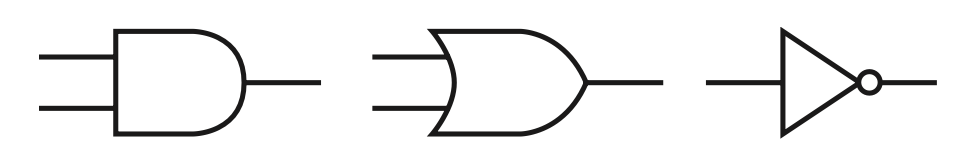
\includegraphics[width=0.5\linewidth]{img/gates.png}%
    }
    \caption{\textit{AND gate, OR gate, and inverter}}
\end{figure}

The gates can be combined to form different forms of logic. An example of this is $\overline{\overline{A} + B}$ which is equivalent to $A \cdot \overline{B}$ by De Morgan's law, seen in \autoref{fig:gates2}.

\begin{figure}[htbp]
    \centering
    \fcolorbox{codeFrame}{white}{
        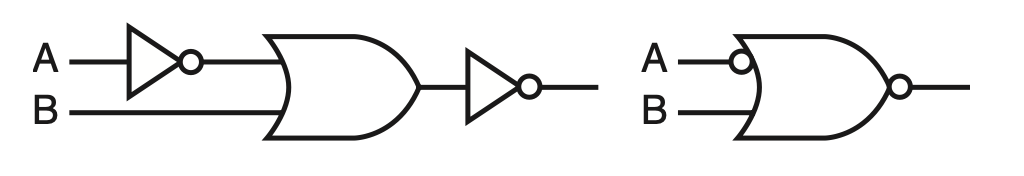
\includegraphics[width=0.5\linewidth]{img/gates2.png}%
    }
    \caption{\textit{Logic gate implementation of example formula}}
    \label{fig:gates2}
\end{figure}

\subsection*{Decoders \& Multiplexors}

A \textbf{decoder} is a logic block that has an n-bit input and $2^n$ outputs, where there is one unique true bit as output from a unique set of bytes of input.

\begin{figure}[htbp]
    \centering
    \fcolorbox{codeFrame}{white}{
        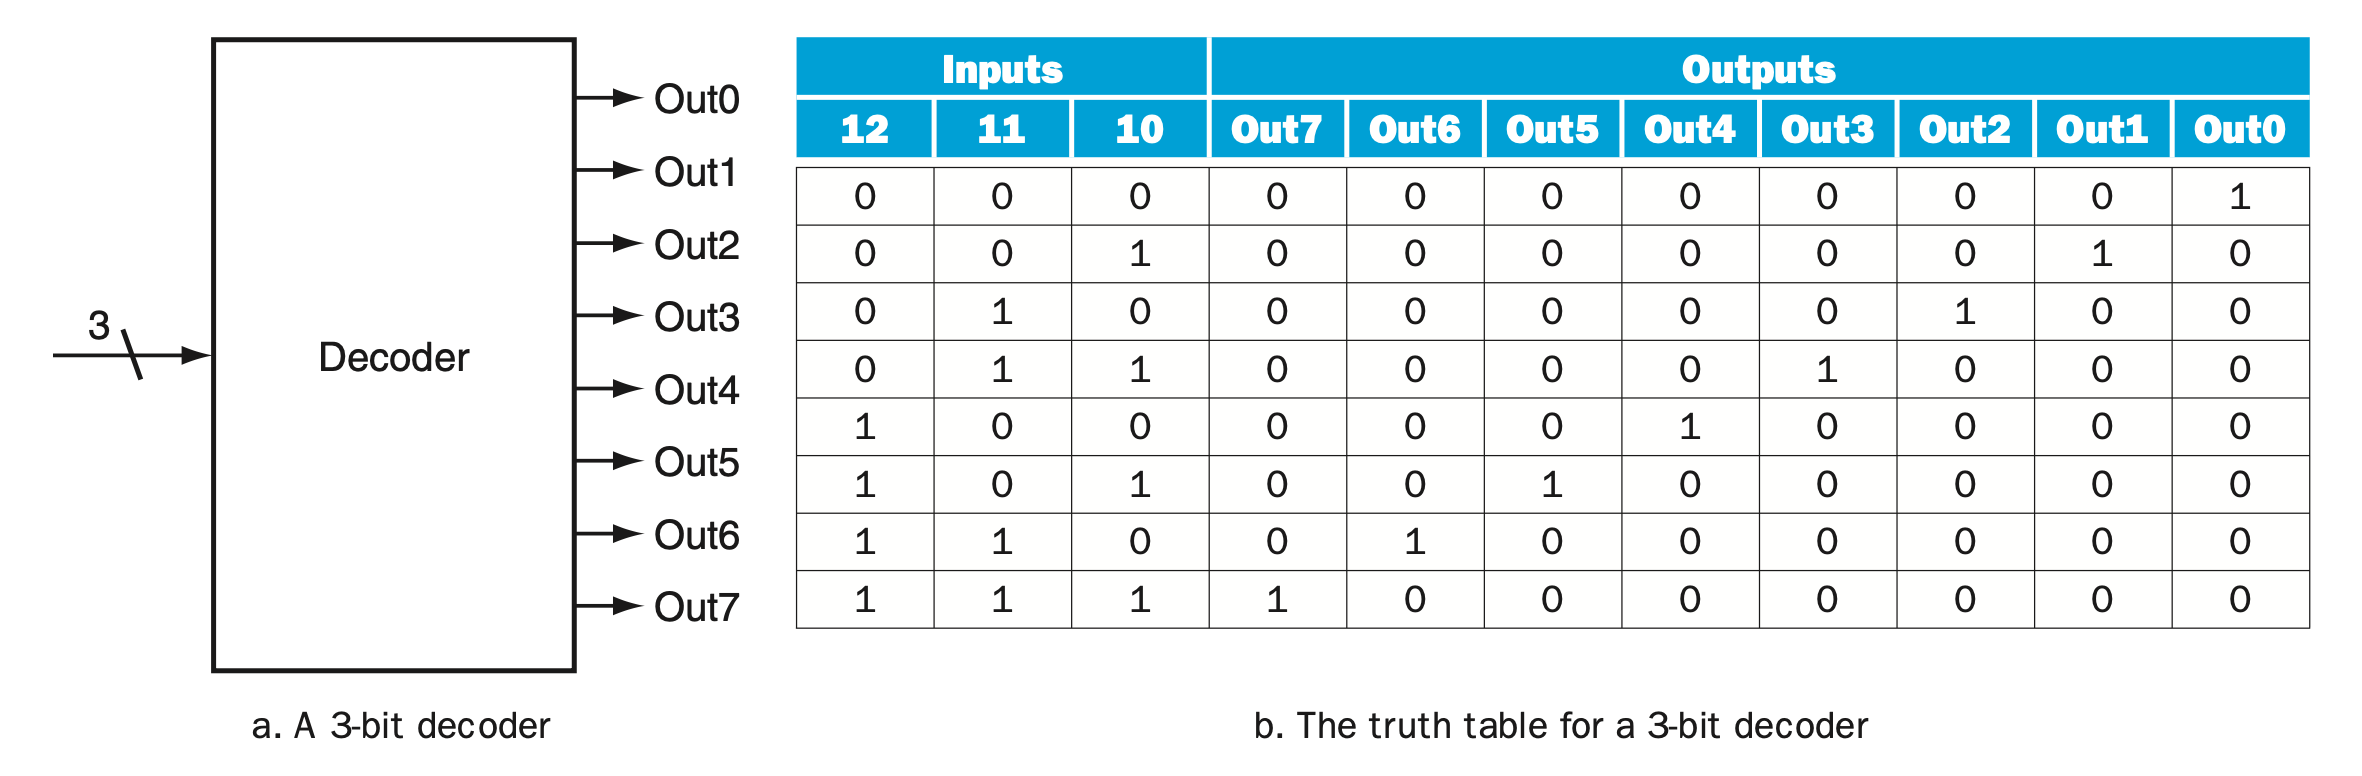
\includegraphics[width=0.7\linewidth]{img/decoder1.png}
    }
    \caption{\textit{3-bit input decoder that generates $2^3=8$ different outputs (Out0 – Out7)}}
\end{figure}

$$2^n \text{ outputs} \ \therefore \ \log_2{(\text{output})} = \text{input bits}$$

Encoders are the other way around.

\textbf{Multiplexors} have a selector input (or control value), that will determine which inputs will become outputs.

In the case of the two-input MUX, its representation is the following, $C=(A \cdot \overline{S}) +(B \cdot S)$, using n (data inputs) AND gates, and one OR gate.

\begin{figure}[htbp]
    \centering
    \fcolorbox{codeFrame}{white}{
        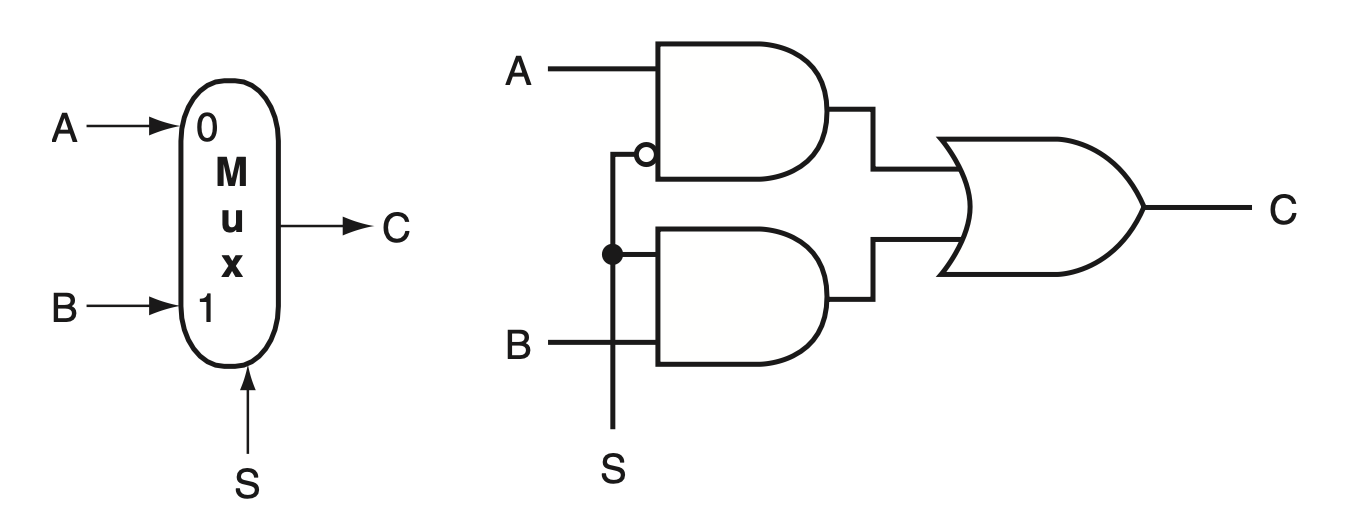
\includegraphics[width=0.5\linewidth]{img/mux1.png}
    }
    \caption{\textit{Two-input multiplexor that generates one output depending on the selector input S}}
\end{figure}

\vspace{-2.5em}
$$n \text{ (data inputs)} \therefore \log_2{n} = S \text{ selector bits required to represent all inputs}$$

Often times a decoder generates n bits for a MUX, to be used as a selector signal.

% \begin{lstlisting}[caption={Simple SIGINT handler}]
% unsigned char stop = 0;
%
% void signal_handler(int x) {
%     stop = 1;
% }
%
% int main(void) {
%     signal(SIGINT, signal_handler);
%
%     /* Pressing Ctrl-C invokes signal_handler() */
%
%     while (!stop);
%     return 0;
% }
% \end{lstlisting}
%
% This is an example of an image.
%
% \begin{figure}[htbp]
%   \centering
%
%   \fcolorbox{codeFrame}{white}{%
%     \includegraphics[width=0.5\linewidth]{img/graph.png}%
%   }
%
%   \caption{My example image}
%   \label{fig:example}
% \end{figure}



\end{document}
